
% Default to the notebook output style

    


% Inherit from the specified cell style.




    
\documentclass[11pt]{article}

    
    
    \usepackage[T1]{fontenc}
    % Nicer default font (+ math font) than Computer Modern for most use cases
    \usepackage{mathpazo}


    % Basic figure setup, for now with no caption control since it's done
    % automatically by Pandoc (which extracts ![](path) syntax from Markdown).
    \usepackage{graphicx}
    % We will generate all images so they have a width \maxwidth. This means
    % that they will get their normal width if they fit onto the page, but
    % are scaled down if they would overflow the margins.
    \makeatletter


    % Ensure that by default, figures have no caption (until we provide a
    % proper Figure object with a Caption API and a way to capture that
    % in the conversion process - todo).
    \usepackage{caption}
    \usepackage{subcaption}

    \usepackage{adjustbox} % Used to constrain images to a maximum size 
    \usepackage{xcolor} % Allow colors to be defined
    \usepackage{enumerate} % Needed for markdown enumerations to work
    \usepackage{geometry} % Used to adjust the document margins
    \usepackage{amsmath} % Equations
    \usepackage{amssymb} % Equations
    \usepackage{textcomp} % defines textquotesingle
    % Hack from http://tex.stackexchange.com/a/47451/13684:
    \AtBeginDocument{%
        \def\PYZsq{\textquotesingle}% Upright quotes in Pygmentized code
    }
    \usepackage{upquote} % Upright quotes for verbatim code
    \usepackage{eurosym} % defines \euro
    \usepackage[mathletters]{ucs} % Extended unicode (utf-8) support
    \usepackage[utf8x]{inputenc} % Allow utf-8 characters in the tex document
    \usepackage{fancyvrb} % verbatim replacement that allows latex
    \usepackage{grffile} % extends the file name processing of package graphics 
                         % to support a larger range 
    % The hyperref package gives us a pdf with properly built
    % internal navigation ('pdf bookmarks' for the table of contents,
    % internal cross-reference links, web links for URLs, etc.)
    \usepackage{hyperref}
    \usepackage{longtable} % longtable support required by pandoc >1.10
    \usepackage{booktabs}  % table support for pandoc > 1.12.2
    \usepackage[inline]{enumitem} % IRkernel/repr support (it uses the enumerate* environment)
    \usepackage[normalem]{ulem} % ulem is needed to support strikethroughs (\sout)
                                % normalem makes italics be italics, not underlines
    \usepackage{mathrsfs}
    

    
    
    % Colors for the hyperref package
    \definecolor{urlcolor}{rgb}{0,.145,.698}
    \definecolor{linkcolor}{rgb}{.71,0.21,0.01}
    \definecolor{citecolor}{rgb}{.12,.54,.11}

    % ANSI colors
    \definecolor{ansi-black}{HTML}{3E424D}
    \definecolor{ansi-black-intense}{HTML}{282C36}
    \definecolor{ansi-red}{HTML}{E75C58}
    \definecolor{ansi-red-intense}{HTML}{B22B31}
    \definecolor{ansi-green}{HTML}{00A250}
    \definecolor{ansi-green-intense}{HTML}{007427}
    \definecolor{ansi-yellow}{HTML}{DDB62B}
    \definecolor{ansi-yellow-intense}{HTML}{B27D12}
    \definecolor{ansi-blue}{HTML}{208FFB}
    \definecolor{ansi-blue-intense}{HTML}{0065CA}
    \definecolor{ansi-magenta}{HTML}{D160C4}
    \definecolor{ansi-magenta-intense}{HTML}{A03196}
    \definecolor{ansi-cyan}{HTML}{60C6C8}
    \definecolor{ansi-cyan-intense}{HTML}{258F8F}
    \definecolor{ansi-white}{HTML}{C5C1B4}
    \definecolor{ansi-white-intense}{HTML}{A1A6B2}
    \definecolor{ansi-default-inverse-fg}{HTML}{FFFFFF}
    \definecolor{ansi-default-inverse-bg}{HTML}{000000}

    % commands and environments needed by pandoc snippets
    % extracted from the output of `pandoc -s`
    \providecommand{\tightlist}{%
      \setlength{\itemsep}{0pt}\setlength{\parskip}{0pt}}
    \DefineVerbatimEnvironment{Highlighting}{Verbatim}{commandchars=\\\{\}}
    % Add ',fontsize=\small' for more characters per line
    \newenvironment{Shaded}{}{}
    \newcommand{\KeywordTok}[1]{\textcolor[rgb]{0.00,0.44,0.13}{\textbf{{#1}}}}
    \newcommand{\DataTypeTok}[1]{\textcolor[rgb]{0.56,0.13,0.00}{{#1}}}
    \newcommand{\DecValTok}[1]{\textcolor[rgb]{0.25,0.63,0.44}{{#1}}}
    \newcommand{\BaseNTok}[1]{\textcolor[rgb]{0.25,0.63,0.44}{{#1}}}
    \newcommand{\FloatTok}[1]{\textcolor[rgb]{0.25,0.63,0.44}{{#1}}}
    \newcommand{\CharTok}[1]{\textcolor[rgb]{0.25,0.44,0.63}{{#1}}}
    \newcommand{\StringTok}[1]{\textcolor[rgb]{0.25,0.44,0.63}{{#1}}}
    \newcommand{\CommentTok}[1]{\textcolor[rgb]{0.38,0.63,0.69}{\textit{{#1}}}}
    \newcommand{\OtherTok}[1]{\textcolor[rgb]{0.00,0.44,0.13}{{#1}}}
    \newcommand{\AlertTok}[1]{\textcolor[rgb]{1.00,0.00,0.00}{\textbf{{#1}}}}
    \newcommand{\FunctionTok}[1]{\textcolor[rgb]{0.02,0.16,0.49}{{#1}}}
    \newcommand{\RegionMarkerTok}[1]{{#1}}
    \newcommand{\ErrorTok}[1]{\textcolor[rgb]{1.00,0.00,0.00}{\textbf{{#1}}}}
    \newcommand{\NormalTok}[1]{{#1}}
    
    % Additional commands for more recent versions of Pandoc
    \newcommand{\ConstantTok}[1]{\textcolor[rgb]{0.53,0.00,0.00}{{#1}}}
    \newcommand{\SpecialCharTok}[1]{\textcolor[rgb]{0.25,0.44,0.63}{{#1}}}
    \newcommand{\VerbatimStringTok}[1]{\textcolor[rgb]{0.25,0.44,0.63}{{#1}}}
    \newcommand{\SpecialStringTok}[1]{\textcolor[rgb]{0.73,0.40,0.53}{{#1}}}
    \newcommand{\ImportTok}[1]{{#1}}
    \newcommand{\DocumentationTok}[1]{\textcolor[rgb]{0.73,0.13,0.13}{\textit{{#1}}}}
    \newcommand{\AnnotationTok}[1]{\textcolor[rgb]{0.38,0.63,0.69}{\textbf{\textit{{#1}}}}}
    \newcommand{\CommentVarTok}[1]{\textcolor[rgb]{0.38,0.63,0.69}{\textbf{\textit{{#1}}}}}
    \newcommand{\VariableTok}[1]{\textcolor[rgb]{0.10,0.09,0.49}{{#1}}}
    \newcommand{\ControlFlowTok}[1]{\textcolor[rgb]{0.00,0.44,0.13}{\textbf{{#1}}}}
    \newcommand{\OperatorTok}[1]{\textcolor[rgb]{0.40,0.40,0.40}{{#1}}}
    \newcommand{\BuiltInTok}[1]{{#1}}
    \newcommand{\ExtensionTok}[1]{{#1}}
    \newcommand{\PreprocessorTok}[1]{\textcolor[rgb]{0.74,0.48,0.00}{{#1}}}
    \newcommand{\AttributeTok}[1]{\textcolor[rgb]{0.49,0.56,0.16}{{#1}}}
    \newcommand{\InformationTok}[1]{\textcolor[rgb]{0.38,0.63,0.69}{\textbf{\textit{{#1}}}}}
    \newcommand{\WarningTok}[1]{\textcolor[rgb]{0.38,0.63,0.69}{\textbf{\textit{{#1}}}}}
    
    
    % Define a nice break command that doesn't care if a line doesn't already
    % exist.
    \def\br{\hspace*{\fill} \\* }
    % Math Jax compatibility definitions
    \def\gt{>}
    \def\lt{<}
    \let\Oldtex\TeX
    \let\Oldlatex\LaTeX
    \renewcommand{\TeX}{\textrm{\Oldtex}}
    \renewcommand{\LaTeX}{\textrm{\Oldlatex}}
    % Document parameters
    % Document title
    \title{Social Media Power: \\
    	    Strategic Targeting for NBA Player Sponsorship}
    \author{Guy Dotan - Stats 404 Final Project}    
    
    
    

    % Pygments definitions
    
\makeatletter
\def\PY@reset{\let\PY@it=\relax \let\PY@bf=\relax%
    \let\PY@ul=\relax \let\PY@tc=\relax%
    \let\PY@bc=\relax \let\PY@ff=\relax}
\def\PY@tok#1{\csname PY@tok@#1\endcsname}
\def\PY@toks#1+{\ifx\relax#1\empty\else%
    \PY@tok{#1}\expandafter\PY@toks\fi}
\def\PY@do#1{\PY@bc{\PY@tc{\PY@ul{%
    \PY@it{\PY@bf{\PY@ff{#1}}}}}}}
\def\PY#1#2{\PY@reset\PY@toks#1+\relax+\PY@do{#2}}

\expandafter\def\csname PY@tok@w\endcsname{\def\PY@tc##1{\textcolor[rgb]{0.73,0.73,0.73}{##1}}}
\expandafter\def\csname PY@tok@c\endcsname{\let\PY@it=\textit\def\PY@tc##1{\textcolor[rgb]{0.25,0.50,0.50}{##1}}}
\expandafter\def\csname PY@tok@cp\endcsname{\def\PY@tc##1{\textcolor[rgb]{0.74,0.48,0.00}{##1}}}
\expandafter\def\csname PY@tok@k\endcsname{\let\PY@bf=\textbf\def\PY@tc##1{\textcolor[rgb]{0.00,0.50,0.00}{##1}}}
\expandafter\def\csname PY@tok@kp\endcsname{\def\PY@tc##1{\textcolor[rgb]{0.00,0.50,0.00}{##1}}}
\expandafter\def\csname PY@tok@kt\endcsname{\def\PY@tc##1{\textcolor[rgb]{0.69,0.00,0.25}{##1}}}
\expandafter\def\csname PY@tok@o\endcsname{\def\PY@tc##1{\textcolor[rgb]{0.40,0.40,0.40}{##1}}}
\expandafter\def\csname PY@tok@ow\endcsname{\let\PY@bf=\textbf\def\PY@tc##1{\textcolor[rgb]{0.67,0.13,1.00}{##1}}}
\expandafter\def\csname PY@tok@nb\endcsname{\def\PY@tc##1{\textcolor[rgb]{0.00,0.50,0.00}{##1}}}
\expandafter\def\csname PY@tok@nf\endcsname{\def\PY@tc##1{\textcolor[rgb]{0.00,0.00,1.00}{##1}}}
\expandafter\def\csname PY@tok@nc\endcsname{\let\PY@bf=\textbf\def\PY@tc##1{\textcolor[rgb]{0.00,0.00,1.00}{##1}}}
\expandafter\def\csname PY@tok@nn\endcsname{\let\PY@bf=\textbf\def\PY@tc##1{\textcolor[rgb]{0.00,0.00,1.00}{##1}}}
\expandafter\def\csname PY@tok@ne\endcsname{\let\PY@bf=\textbf\def\PY@tc##1{\textcolor[rgb]{0.82,0.25,0.23}{##1}}}
\expandafter\def\csname PY@tok@nv\endcsname{\def\PY@tc##1{\textcolor[rgb]{0.10,0.09,0.49}{##1}}}
\expandafter\def\csname PY@tok@no\endcsname{\def\PY@tc##1{\textcolor[rgb]{0.53,0.00,0.00}{##1}}}
\expandafter\def\csname PY@tok@nl\endcsname{\def\PY@tc##1{\textcolor[rgb]{0.63,0.63,0.00}{##1}}}
\expandafter\def\csname PY@tok@ni\endcsname{\let\PY@bf=\textbf\def\PY@tc##1{\textcolor[rgb]{0.60,0.60,0.60}{##1}}}
\expandafter\def\csname PY@tok@na\endcsname{\def\PY@tc##1{\textcolor[rgb]{0.49,0.56,0.16}{##1}}}
\expandafter\def\csname PY@tok@nt\endcsname{\let\PY@bf=\textbf\def\PY@tc##1{\textcolor[rgb]{0.00,0.50,0.00}{##1}}}
\expandafter\def\csname PY@tok@nd\endcsname{\def\PY@tc##1{\textcolor[rgb]{0.67,0.13,1.00}{##1}}}
\expandafter\def\csname PY@tok@s\endcsname{\def\PY@tc##1{\textcolor[rgb]{0.73,0.13,0.13}{##1}}}
\expandafter\def\csname PY@tok@sd\endcsname{\let\PY@it=\textit\def\PY@tc##1{\textcolor[rgb]{0.73,0.13,0.13}{##1}}}
\expandafter\def\csname PY@tok@si\endcsname{\let\PY@bf=\textbf\def\PY@tc##1{\textcolor[rgb]{0.73,0.40,0.53}{##1}}}
\expandafter\def\csname PY@tok@se\endcsname{\let\PY@bf=\textbf\def\PY@tc##1{\textcolor[rgb]{0.73,0.40,0.13}{##1}}}
\expandafter\def\csname PY@tok@sr\endcsname{\def\PY@tc##1{\textcolor[rgb]{0.73,0.40,0.53}{##1}}}
\expandafter\def\csname PY@tok@ss\endcsname{\def\PY@tc##1{\textcolor[rgb]{0.10,0.09,0.49}{##1}}}
\expandafter\def\csname PY@tok@sx\endcsname{\def\PY@tc##1{\textcolor[rgb]{0.00,0.50,0.00}{##1}}}
\expandafter\def\csname PY@tok@m\endcsname{\def\PY@tc##1{\textcolor[rgb]{0.40,0.40,0.40}{##1}}}
\expandafter\def\csname PY@tok@gh\endcsname{\let\PY@bf=\textbf\def\PY@tc##1{\textcolor[rgb]{0.00,0.00,0.50}{##1}}}
\expandafter\def\csname PY@tok@gu\endcsname{\let\PY@bf=\textbf\def\PY@tc##1{\textcolor[rgb]{0.50,0.00,0.50}{##1}}}
\expandafter\def\csname PY@tok@gd\endcsname{\def\PY@tc##1{\textcolor[rgb]{0.63,0.00,0.00}{##1}}}
\expandafter\def\csname PY@tok@gi\endcsname{\def\PY@tc##1{\textcolor[rgb]{0.00,0.63,0.00}{##1}}}
\expandafter\def\csname PY@tok@gr\endcsname{\def\PY@tc##1{\textcolor[rgb]{1.00,0.00,0.00}{##1}}}
\expandafter\def\csname PY@tok@ge\endcsname{\let\PY@it=\textit}
\expandafter\def\csname PY@tok@gs\endcsname{\let\PY@bf=\textbf}
\expandafter\def\csname PY@tok@gp\endcsname{\let\PY@bf=\textbf\def\PY@tc##1{\textcolor[rgb]{0.00,0.00,0.50}{##1}}}
\expandafter\def\csname PY@tok@go\endcsname{\def\PY@tc##1{\textcolor[rgb]{0.53,0.53,0.53}{##1}}}
\expandafter\def\csname PY@tok@gt\endcsname{\def\PY@tc##1{\textcolor[rgb]{0.00,0.27,0.87}{##1}}}
\expandafter\def\csname PY@tok@err\endcsname{\def\PY@bc##1{\setlength{\fboxsep}{0pt}\fcolorbox[rgb]{1.00,0.00,0.00}{1,1,1}{\strut ##1}}}
\expandafter\def\csname PY@tok@kc\endcsname{\let\PY@bf=\textbf\def\PY@tc##1{\textcolor[rgb]{0.00,0.50,0.00}{##1}}}
\expandafter\def\csname PY@tok@kd\endcsname{\let\PY@bf=\textbf\def\PY@tc##1{\textcolor[rgb]{0.00,0.50,0.00}{##1}}}
\expandafter\def\csname PY@tok@kn\endcsname{\let\PY@bf=\textbf\def\PY@tc##1{\textcolor[rgb]{0.00,0.50,0.00}{##1}}}
\expandafter\def\csname PY@tok@kr\endcsname{\let\PY@bf=\textbf\def\PY@tc##1{\textcolor[rgb]{0.00,0.50,0.00}{##1}}}
\expandafter\def\csname PY@tok@bp\endcsname{\def\PY@tc##1{\textcolor[rgb]{0.00,0.50,0.00}{##1}}}
\expandafter\def\csname PY@tok@fm\endcsname{\def\PY@tc##1{\textcolor[rgb]{0.00,0.00,1.00}{##1}}}
\expandafter\def\csname PY@tok@vc\endcsname{\def\PY@tc##1{\textcolor[rgb]{0.10,0.09,0.49}{##1}}}
\expandafter\def\csname PY@tok@vg\endcsname{\def\PY@tc##1{\textcolor[rgb]{0.10,0.09,0.49}{##1}}}
\expandafter\def\csname PY@tok@vi\endcsname{\def\PY@tc##1{\textcolor[rgb]{0.10,0.09,0.49}{##1}}}
\expandafter\def\csname PY@tok@vm\endcsname{\def\PY@tc##1{\textcolor[rgb]{0.10,0.09,0.49}{##1}}}
\expandafter\def\csname PY@tok@sa\endcsname{\def\PY@tc##1{\textcolor[rgb]{0.73,0.13,0.13}{##1}}}
\expandafter\def\csname PY@tok@sb\endcsname{\def\PY@tc##1{\textcolor[rgb]{0.73,0.13,0.13}{##1}}}
\expandafter\def\csname PY@tok@sc\endcsname{\def\PY@tc##1{\textcolor[rgb]{0.73,0.13,0.13}{##1}}}
\expandafter\def\csname PY@tok@dl\endcsname{\def\PY@tc##1{\textcolor[rgb]{0.73,0.13,0.13}{##1}}}
\expandafter\def\csname PY@tok@s2\endcsname{\def\PY@tc##1{\textcolor[rgb]{0.73,0.13,0.13}{##1}}}
\expandafter\def\csname PY@tok@sh\endcsname{\def\PY@tc##1{\textcolor[rgb]{0.73,0.13,0.13}{##1}}}
\expandafter\def\csname PY@tok@s1\endcsname{\def\PY@tc##1{\textcolor[rgb]{0.73,0.13,0.13}{##1}}}
\expandafter\def\csname PY@tok@mb\endcsname{\def\PY@tc##1{\textcolor[rgb]{0.40,0.40,0.40}{##1}}}
\expandafter\def\csname PY@tok@mf\endcsname{\def\PY@tc##1{\textcolor[rgb]{0.40,0.40,0.40}{##1}}}
\expandafter\def\csname PY@tok@mh\endcsname{\def\PY@tc##1{\textcolor[rgb]{0.40,0.40,0.40}{##1}}}
\expandafter\def\csname PY@tok@mi\endcsname{\def\PY@tc##1{\textcolor[rgb]{0.40,0.40,0.40}{##1}}}
\expandafter\def\csname PY@tok@il\endcsname{\def\PY@tc##1{\textcolor[rgb]{0.40,0.40,0.40}{##1}}}
\expandafter\def\csname PY@tok@mo\endcsname{\def\PY@tc##1{\textcolor[rgb]{0.40,0.40,0.40}{##1}}}
\expandafter\def\csname PY@tok@ch\endcsname{\let\PY@it=\textit\def\PY@tc##1{\textcolor[rgb]{0.25,0.50,0.50}{##1}}}
\expandafter\def\csname PY@tok@cm\endcsname{\let\PY@it=\textit\def\PY@tc##1{\textcolor[rgb]{0.25,0.50,0.50}{##1}}}
\expandafter\def\csname PY@tok@cpf\endcsname{\let\PY@it=\textit\def\PY@tc##1{\textcolor[rgb]{0.25,0.50,0.50}{##1}}}
\expandafter\def\csname PY@tok@c1\endcsname{\let\PY@it=\textit\def\PY@tc##1{\textcolor[rgb]{0.25,0.50,0.50}{##1}}}
\expandafter\def\csname PY@tok@cs\endcsname{\let\PY@it=\textit\def\PY@tc##1{\textcolor[rgb]{0.25,0.50,0.50}{##1}}}

\def\PYZbs{\char`\\}
\def\PYZus{\char`\_}
\def\PYZob{\char`\{}
\def\PYZcb{\char`\}}
\def\PYZca{\char`\^}
\def\PYZam{\char`\&}
\def\PYZlt{\char`\<}
\def\PYZgt{\char`\>}
\def\PYZsh{\char`\#}
\def\PYZpc{\char`\%}
\def\PYZdl{\char`\$}
\def\PYZhy{\char`\-}
\def\PYZsq{\char`\'}
\def\PYZdq{\char`\"}
\def\PYZti{\char`\~}
% for compatibility with earlier versions
\def\PYZat{@}
\def\PYZlb{[}
\def\PYZrb{]}
\makeatother


    % Exact colors from NB
    \definecolor{incolor}{rgb}{0.0, 0.0, 0.5}
    \definecolor{outcolor}{rgb}{0.545, 0.0, 0.0}



    
    % Prevent overflowing lines due to hard-to-break entities
    \sloppy 
    % Setup hyperref package
    \hypersetup{
      breaklinks=true,  % so long urls are correctly broken across lines
      colorlinks=true,
      urlcolor=urlcolor,
      linkcolor=linkcolor,
      citecolor=citecolor,
      }
    % Slightly bigger margins than the latex defaults
    
    \geometry{verbose,tmargin=1in,bmargin=1in,lmargin=1in,rmargin=1in}
    
    

    \begin{document}
    
    
    \maketitle
    


    \section{Setting the Stage}\label{setting-the-stage}

Sponsorships are as deeply integrated into the fabric of the sports
landscape as the very players and competition itself. Every year around
the world, billions of dollars are being invested into professional
athletes for brand promotion. Sports stars are some of the strongest
marketing influencers of any celebrity, but over the past few years
trends have shifted dramatically in this industry. All of the world's
biggest sporting competitions (NFL, NBA, Premier League, etc.) are
reporting declining numbers of traditional TV viewers. That said, the
sports sponsorship market remains as strong as ever due to the explosion
in social media engagement.

With the focus of sports branding shifting toward social media,
marketers need to focus their attention on these platforms. Of all the
major sports leagues in America, the NBA is growing the fastest and is
the most progressive at integrating and promoting social media. As shown
below the top three yearly endorsement contracts in the NBA are valued
at over \$35 million (per
\href{https://kaggle.com/noahgift/social-power-nba}{Kaggle's} social
power dataset). In addition to the contractional endorsements, NBA
stars are able to generate brand exposure organically through social
media. Using proprietary computer vision technology,
\href{https://www.gumgum.com/sports}{GumGum Sports}, is able to track
brand exposures across social media and attribute a corresponding media
value. So far in the 2018-19 NBA season, LeBron James leads all players
by generating almost \$5.0 million of organic sponsorship content
through Twitter, Instagram, and Facebook.

\begin{figure}[h]
\centering
 \adjustimage{max size={0.85\linewidth}}{sponsorship_landscape.png}
 \label{}
\caption{}
\end{figure}

The relationship between the NBA and Twitter continues to grow as does
the value brought in by that platform. With all of this data surrounding
the power in valuing the NBA and social media, an important question
emerges. \textbf{How should a brand/agency strategically determine the best
players to target for sponsorships?}


    \section{The Data}\label{the-data}

    In order to build a model that can identify NBA players with high social
media value potential I pulled a dataset from Kaggle regarding the
2016-17 NBA season. The data includes a variety of on-the-court
basketball statistics along with some social media metrics. Included
were about 40 variables. The relevant variables in our dataset are grouped into the following
categories:


\textbf{Potential Input Variables:}
\begin{itemize}
\tightlist
\item 26 basic statistics (PPG, 3PM, FG\%, etc.)
\item  6 advanced statistics (ORPM, DRPM, PIE, etc.)
\item  6 other metrics (Age, Position, Wikipedia Page Views, etc.)
\end{itemize}

\textbf{Potential Output Variables:}
\begin{itemize}
\tightlist
\item Twitter Retweet Count
\item Twitter Favorite Count
\end{itemize}

Before we begin to handle any missing values and potential issues with
the dataset the goal is to determine on a high-level how we want to
structure this model. For the target output variable we determined that
\textbf{Twitter retweets} was the better metric to reflect social media
influence. Retweets show a much more active engagement with media
content than favoriting does and therefore would generate more brand
value. In addition retweeting would spread that content to that user's
network of followers which increases the original exposure even further.

As for the input variables, the goal of this exercise would be to
develop a model that could use widely available data (basketball stats)
to predict a more difficult to aquire and valuable metric as social
media engagement. Therefore, we will focus our attention on the
numerical basketball and team statistics. Right off the bat this
eliminates position, player name, team name, and wikipedia page views.

    \section{Data Processing}\label{data-processing}

\subsection{Null values}\label{null-values}

First step toward handling our data was to resolve issues with null
values. As shown below, only four columns had any null values. In cases
where 3PT\% and FT\% were null, this was due to the player having taken
no FT or 3PT attempts. As a result, we set these values equal to 0. In
cases where Twitter Retweet and Favorite Count were null, we
unfortunately had to remove those players as we needed this value to be our output metric.


    \begin{Verbatim}[commandchars=\\\{\}]
3P\%                       7
FT\%                       2
TWITTER\_FAVORITE\_COUNT    3
TWITTER\_RETWEET\_COUNT     3
dtype: int64

    \end{Verbatim}

        
\begin{table}[h]
\begin{tabular}{@{}lllllllll@{}}
\toprule
PLAYER           & 3P  & 3PA & 3P\%  & FT  & FTA & FT\%  & TWIT\_FAV\_CT & TWIT\_RETWEET\_CT \\ \midrule
Tyson Chandler   & 0   & 0   & null   & 1.9 & 2.6 & 0.734 & 29                       & 9                       \\
David Lee        & 0   & 0   & null   & 1   & 1.4 & 0.708 & 56.5                     & 35                      \\
Ian Mahinmi      & 0   & 0   & null   & 1.4 & 2.4 & 0.573 & 10                       & 5                       \\
Anthony Brown    & 0.6 & 2.5 & 0.259 & 0   & 0   & null   & 3                        & 3                       \\
Dragan Bender    & 0.7 & 2.3 & 0.277 & 0.1 & 0.3 & 0.364 & null                      & null                     \\
Omer Asik        & 0   & 0   & null   & 0.7 & 1.3 & 0.59  & null                      & null                     \\
Miles Plumlee    & 0   & 0   & null   & 0.6 & 0.9 & 0.641 & 11                       & 3                       \\
Rakeem Christmas & 0   & 0   & null   & 0.7 & 1   & 0.724 & 13                       & 3                       \\
Cole Aldrich     & 0   & 0   & null   & 0.2 & 0.4 & 0.682 & 22                       & 9                       \\
Bruno Caboclo    & 0.2 & 0.7 & 0.333 & 0   & 0   & null   & 11                       & 8                       \\
Alonzo Gee       & 0   & 0.2 & 0     & 0.4 & 0.7 & 0.556 & null                      & null                     \\ \bottomrule
\end{tabular}
\end{table}

    
    \subsection{Binning retweets}\label{binning-retweets}

The second step needed in our data processing was to bin our output
variable into larger buckets. For the purposes of our model it is not
necessary to predict exactly how many retweets a player would have.
Instead we just need to know the general range.


\begin{Verbatim}[commandchars=\\\{\}]
{\color{outcolor}Out[{\color{outcolor}185}]:} 10-50     95
          <10       82
          50-150    34
          150+      25
          Name: TWEET\_CAT, dtype: int64
\end{Verbatim}
            
    \section{Modeling Approach}\label{modeling-approach}

Before we begin to model our dataset, there was something to note about
our input variables. One notable intricacy about the dataset is many of
the advanced basketball statistics are a combination of the basic
statistics. As a result there would be much covariance between these
features. As a result we decided to narrow the feature set to just seven
key metrics.

With the features determined, we decided to utilize the random forest
modeling technique to predict which players fall into which retweet
count bucket. After splitting the data into a 75-25 train-test set split we
ran a random forest with up to 2500 trees, using a minimum leaf sample
of 5, and balanced weight sampling.

As shown below we saw that the optimal OOB error occured at 1500 trees.
In addition our feature importance plot showcased PIE (Player Inpact
Estimate) and Salary (millions) as the most prominent features.

\pagebreak

\begin{centering}
\begin{figure}[h]
  \begin{subfigure}[b]{0.4\textwidth}
    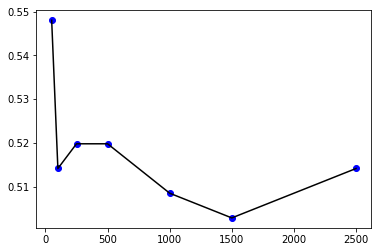
\includegraphics[width=\textwidth]{output_12_0.png}
    \caption{OOB Error Plot}
    \label{fig:1}
  \end{subfigure}
  \hfill
  \begin{subfigure}[b]{0.4\textwidth}
    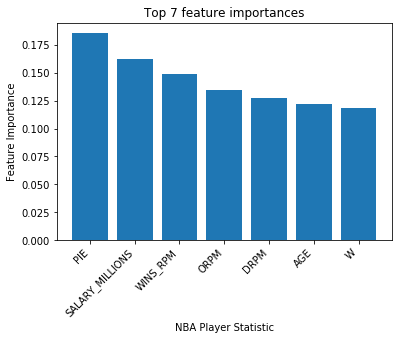
\includegraphics[width=\textwidth]{output_13_0.png}
    \caption{Feature Importance Plot}
    \label{fig:1}
  \end{subfigure}
\end{figure}
\end{centering}



    \section{Key Findings}\label{key-findings}

The last step with analyzing our random forest model was to take a look
at the prediction success. When applying our model to our validation set
of 59 NBA players, our model accurately predicted the retweet bucket in
just under half those cases (\textasciitilde{}47\%). The prediction
results are displayed below in the confusion matrix.
    
    \begin{verbatim}
        <10  10-50  50-150  150+
<10      12      1       2     9
10-50     1      1       4     0
50-150    0      3       3     3
150+      7      0       1    12
    \end{verbatim}

    
    \begin{Verbatim}[commandchars=\\\{\}]
{\color{incolor}In [{\color{incolor}176}]:} \PY{n}{accuracy\PYZus{}score}\PY{p}{(}\PY{n}{y\PYZus{}valid}\PY{p}{,} \PY{n}{y\PYZus{}pred\PYZus{}valid}\PY{p}{)}
\end{Verbatim}

\begin{Verbatim}[commandchars=\\\{\}]
{\color{outcolor}Out[{\color{outcolor}176}]:} 0.4745762711864407
\end{Verbatim}
            
    \section{Use Cases}\label{use-cases}

Building a model that can predict an NBA's player's social media
presence could be an extremely powerful tool for a brand or sponsorship
agency. There could be a lot of untapped value potential in emerging NBA
players and being able to identify those players would be critical. The
following would be just a few use cases on how to utilize this model's
potential.

\subsection{Targeting Rookies}\label{targeting-rookies}

\begin{itemize}
\tightlist
\item
  With all rookies up for grabs after declaring for NBA draft, brands
  must determine which ones target with somewhat limited of information.
\item
  By plugging in the rookie's NCAA statistics, rookie salary, and
  drafted team a branding agency could predict the social media power of
  the next great NBA star.
\end{itemize}

\subsection{Trades / Free Agency}\label{trades-free-agency}

\begin{itemize}
\tightlist
\item
  As one would expect, changing teams can significantly affect a
  player's social media presence.
\item
  Joining a top tier team could mean performing on a better team that
  would play more nationally televised games and postseason games. But
  joining a lower tier team could make the player the focal point of the
  franchise and also increase value.
\item
  Also, joining a team in a bigger markets would obviously lead to
  increased exposure as well.
\end{itemize}

\subsection{New Contracts}\label{new-contracts}

\begin{itemize}
\tightlist
\item
  Our model indicated that player salary was a top feature in predicting
  social media power.
\item
  Targeting NBA players with a big pay raise in the offseason gives a
  major indication into the increase in social media value
\end{itemize}

    \section{Future Research}\label{future-research}

\subsection{Instagram and Facebook}\label{instagram-and-facebook}

Although Twitter is the most active of the three social media platforms
among NBA players, it is mainly a text-driven platform. Instagram and
Facebook generate far more visual media (images and videos) and therfore
would provide far more opportunities for product placement. For a more
complete analysis of the power of social media sponsorships, both
Instagrm and Facebook must be included.

\subsection{Attendance}\label{attendance}

We know that the team plays a major role in a player's marketing power.
There are many ways to attempt to quantify a team's impact. One of the
most transparent methods would be to incoporate team attendence into the
model. Attendence indicates not only how many eyes are at the game but
also directly correlates with the size of the TV and social media
market.

\subsection{Season-to-Season Trends}\label{season-to-season-trends}

This model was weakened by the fact that we are only working with a
single season's worth of data. In order to build a more robust model,
increasing the size of the dataset would be crucial. Not only would
having more data points increase the quality of the model but it would
also unable use to examine player trends. If an NBA player's stats seems
to be improving year over year then we would assume his social media
precense to follow a similar positive trajectory.

\subsection{Postseason performance}\label{postseason-performance}

Finally, our dataset was limited to regular season statistics. The NBA
playoff brings in millions of dollars every season just through
broadcasting rights. NBA players who perform in the playoffs and perform
well experience vast increases in their exposure. An analysis of the
branding value of an NBA player would not be complete without examining
their playoff metrics as well.

\pagebreak

\section{Appdendix}

\subsection{Data Loading and Processing code}

    \begin{Verbatim}[commandchars=\\\{\}]
{\color{incolor}In [{\color{incolor}165}]:} \PY{k+kn}{import} \PY{n+nn}{pandas} \PY{k}{as} \PY{n+nn}{pd}
          \PY{k+kn}{import} \PY{n+nn}{numpy} \PY{k}{as} \PY{n+nn}{np}
          \PY{k+kn}{import} \PY{n+nn}{random}
          \PY{k+kn}{from} \PY{n+nn}{sklearn}\PY{n+nn}{.}\PY{n+nn}{model\PYZus{}selection} \PY{k}{import} \PY{n}{train\PYZus{}test\PYZus{}split}
          \PY{k+kn}{from} \PY{n+nn}{sklearn}\PY{n+nn}{.}\PY{n+nn}{ensemble} \PY{k}{import} \PY{n}{RandomForestClassifier}
          \PY{k+kn}{import} \PY{n+nn}{matplotlib}\PY{n+nn}{.}\PY{n+nn}{pyplot} \PY{k}{as} \PY{n+nn}{plt}
          \PY{k+kn}{from} \PY{n+nn}{sklearn}\PY{n+nn}{.}\PY{n+nn}{metrics} \PY{k}{import} \PY{n}{accuracy\PYZus{}score}\PY{p}{,} \PY{n}{confusion\PYZus{}matrix}
          
          \PY{n}{PATH} \PY{o}{=} \PY{p}{(}\PY{l+s+s1}{\PYZsq{}}\PY{l+s+s1}{https://s3\PYZhy{}us\PYZhy{}west\PYZhy{}1.amazonaws.com/uclastats404\PYZhy{}project/}\PY{l+s+s1}{\PYZsq{}}
                      \PY{l+s+s1}{\PYZsq{}}\PY{l+s+s1}{nba\PYZus{}2017\PYZus{}players\PYZus{}with\PYZus{}salary\PYZus{}wiki\PYZus{}twitter.csv}\PY{l+s+s1}{\PYZsq{}}\PY{p}{)}
          \PY{n}{DF} \PY{o}{=} \PY{n}{pd}\PY{o}{.}\PY{n}{read\PYZus{}csv}\PY{p}{(}\PY{n}{PATH}\PY{p}{)}
\end{Verbatim}

  \begin{Verbatim}[commandchars=\\\{\}]
{\color{incolor}In [{\color{incolor}151}]:} \PY{n}{null\PYZus{}columns}\PY{o}{=}\PY{n}{DF}\PY{o}{.}\PY{n}{columns}\PY{p}{[}\PY{n}{DF}\PY{o}{.}\PY{n}{isnull}\PY{p}{(}\PY{p}{)}\PY{o}{.}\PY{n}{any}\PY{p}{(}\PY{p}{)}\PY{p}{]}
          \PY{n+nb}{print}\PY{p}{(}\PY{n}{DF}\PY{p}{[}\PY{n}{null\PYZus{}columns}\PY{p}{]}\PY{o}{.}\PY{n}{isnull}\PY{p}{(}\PY{p}{)}\PY{o}{.}\PY{n}{sum}\PY{p}{(}\PY{p}{)}\PY{p}{)}    
          \PY{n}{df\PYZus{}subset} \PY{o}{=} \PY{n}{DF}\PY{p}{[}\PY{p}{[}\PY{l+s+s2}{\PYZdq{}}\PY{l+s+s2}{PLAYER}\PY{l+s+s2}{\PYZdq{}}\PY{p}{,}\PY{l+s+s2}{\PYZdq{}}\PY{l+s+s2}{3P}\PY{l+s+s2}{\PYZdq{}}\PY{p}{,}\PY{l+s+s2}{\PYZdq{}}\PY{l+s+s2}{3PA}\PY{l+s+s2}{\PYZdq{}}\PY{p}{,}\PY{l+s+s2}{\PYZdq{}}\PY{l+s+s2}{3P}\PY{l+s+s2}{\PYZpc{}}\PY{l+s+s2}{\PYZdq{}}\PY{p}{,}\PY{l+s+s2}{\PYZdq{}}\PY{l+s+s2}{FT}\PY{l+s+s2}{\PYZdq{}}\PY{p}{,}\PY{l+s+s2}{\PYZdq{}}\PY{l+s+s2}{FTA}\PY{l+s+s2}{\PYZdq{}}\PY{p}{,}\PY{l+s+s2}{\PYZdq{}}\PY{l+s+s2}{FT}\PY{l+s+s2}{\PYZpc{}}\PY{l+s+s2}{\PYZdq{}}\PY{p}{,}
                          \PY{l+s+s2}{\PYZdq{}}\PY{l+s+s2}{TWITTER\PYZus{}FAVORITE\PYZus{}COUNT}\PY{l+s+s2}{\PYZdq{}}\PY{p}{,}\PY{l+s+s2}{\PYZdq{}}\PY{l+s+s2}{TWITTER\PYZus{}RETWEET\PYZus{}COUNT}\PY{l+s+s2}{\PYZdq{}}\PY{p}{]}\PY{p}{]}
          \PY{n}{display}\PY{p}{(}\PY{n}{df\PYZus{}subset}\PY{p}{[}\PY{n}{DF}\PY{o}{.}\PY{n}{isnull}\PY{p}{(}\PY{p}{)}\PY{o}{.}\PY{n}{any}\PY{p}{(}\PY{n}{axis}\PY{o}{=}\PY{l+m+mi}{1}\PY{p}{)}\PY{p}{]}\PY{p}{)}
          \PY{n}{nba} \PY{o}{=} \PY{n}{DF}\PY{p}{[}\PY{n}{np}\PY{o}{.}\PY{n}{isfinite}\PY{p}{(}\PY{n}{DF}\PY{p}{[}\PY{l+s+s1}{\PYZsq{}}\PY{l+s+s1}{TWITTER\PYZus{}RETWEET\PYZus{}COUNT}\PY{l+s+s1}{\PYZsq{}}\PY{p}{]}\PY{p}{)}\PY{p}{]}
\end{Verbatim}

\subsection{Binning Code}

    \begin{Verbatim}[commandchars=\\\{\}]
{\color{incolor}In [{\color{incolor}185}]:} \PY{k}{def} \PY{n+nf}{bin\PYZus{}retweet\PYZus{}count}\PY{p}{(}\PY{n}{retweets}\PY{p}{:} \PY{n+nb}{float}\PY{p}{)} \PY{o}{\PYZhy{}}\PY{o}{\PYZgt{}} \PY{n+nb}{str}\PY{p}{:}
              \PY{k}{if} \PY{n}{retweets} \PY{o}{\PYZlt{}} \PY{l+m+mi}{10}\PY{p}{:}
                  \PY{n}{retweet\PYZus{}cat\PYZus{}group} \PY{o}{=} \PY{l+s+s2}{\PYZdq{}}\PY{l+s+s2}{\PYZlt{}10}\PY{l+s+s2}{\PYZdq{}}
              \PY{k}{elif} \PY{p}{(}\PY{n}{retweets} \PY{o}{\PYZgt{}}\PY{o}{=} \PY{l+m+mi}{10}\PY{p}{)} \PY{o}{\PYZam{}} \PY{p}{(}\PY{n}{retweets} \PY{o}{\PYZlt{}} \PY{l+m+mi}{50}\PY{p}{)}\PY{p}{:}
                  \PY{n}{retweet\PYZus{}cat\PYZus{}group} \PY{o}{=} \PY{l+s+s2}{\PYZdq{}}\PY{l+s+s2}{10\PYZhy{}50}\PY{l+s+s2}{\PYZdq{}}
              \PY{k}{elif} \PY{p}{(}\PY{n}{retweets} \PY{o}{\PYZgt{}}\PY{o}{=} \PY{l+m+mi}{50}\PY{p}{)} \PY{o}{\PYZam{}} \PY{p}{(}\PY{n}{retweets} \PY{o}{\PYZlt{}} \PY{l+m+mi}{150}\PY{p}{)}\PY{p}{:}
                  \PY{n}{retweet\PYZus{}cat\PYZus{}group} \PY{o}{=} \PY{l+s+s2}{\PYZdq{}}\PY{l+s+s2}{50\PYZhy{}150}\PY{l+s+s2}{\PYZdq{}}
              \PY{k}{else}\PY{p}{:}
                  \PY{n}{retweet\PYZus{}cat\PYZus{}group} \PY{o}{=} \PY{l+s+s2}{\PYZdq{}}\PY{l+s+s2}{150+}\PY{l+s+s2}{\PYZdq{}}
              \PY{k}{return} \PY{n}{retweet\PYZus{}cat\PYZus{}group}
          
          \PY{c+c1}{\PYZsh{} prevent pandas warning message for SettingWithCopyWarning}
          \PY{c+c1}{\PYZsh{} taken from https://stackoverflow.com/questions/20625582/}
              \PY{c+c1}{\PYZsh{} how\PYZhy{}to\PYZhy{}deal\PYZhy{}with\PYZhy{}settingwithcopywarning\PYZhy{}in\PYZhy{}pandas}
          \PY{n}{pd}\PY{o}{.}\PY{n}{options}\PY{o}{.}\PY{n}{mode}\PY{o}{.}\PY{n}{chained\PYZus{}assignment} \PY{o}{=} \PY{k+kc}{None}
          \PY{n}{nba}\PY{p}{[}\PY{l+s+s1}{\PYZsq{}}\PY{l+s+s1}{TWEET\PYZus{}CAT}\PY{l+s+s1}{\PYZsq{}}\PY{p}{]} \PY{o}{=} \PY{n}{nba}\PY{p}{[}\PY{l+s+s1}{\PYZsq{}}\PY{l+s+s1}{TWITTER\PYZus{}RETWEET\PYZus{}COUNT}\PY{l+s+s1}{\PYZsq{}}\PY{p}{]}\PY{o}{.}\PY{n}{apply}\PY{p}{(}\PY{k}{lambda}
                                                                \PY{n}{x}\PY{p}{:} \PY{n}{bin\PYZus{}retweet\PYZus{}count}\PY{p}{(}\PY{n}{x}\PY{p}{)}\PY{p}{)}
          \PY{n}{nba}\PY{p}{[}\PY{l+s+s1}{\PYZsq{}}\PY{l+s+s1}{TWEET\PYZus{}CAT}\PY{l+s+s1}{\PYZsq{}}\PY{p}{]}\PY{o}{.}\PY{n}{value\PYZus{}counts}\PY{p}{(}\PY{p}{)}
\end{Verbatim}

\pagebreak

\subsection{Random Forest Code}

    \begin{Verbatim}[commandchars=\\\{\}]
{\color{incolor}In [{\color{incolor}179}]:} \PY{n}{df\PYZus{}train}\PY{p}{,} \PY{n}{df\PYZus{}valid} \PY{o}{=} \PY{n}{train\PYZus{}test\PYZus{}split}\PY{p}{(}\PY{n}{nba}\PY{p}{,}
                                                \PY{n}{test\PYZus{}size}\PY{o}{=}\PY{l+m+mf}{0.25}\PY{p}{,}
                                                \PY{n}{random\PYZus{}state}\PY{o}{=}\PY{l+m+mi}{2019}\PY{p}{,}
                                                \PY{n}{stratify}\PY{o}{=}\PY{n}{nba}\PY{p}{[}\PY{l+s+s1}{\PYZsq{}}\PY{l+s+s1}{TWEET\PYZus{}CAT}\PY{l+s+s1}{\PYZsq{}}\PY{p}{]}\PY{p}{)}
          
          \PY{n}{y} \PY{o}{=} \PY{n}{df\PYZus{}train}\PY{p}{[}\PY{l+s+s1}{\PYZsq{}}\PY{l+s+s1}{TWEET\PYZus{}CAT}\PY{l+s+s1}{\PYZsq{}}\PY{p}{]}
          \PY{n}{X} \PY{o}{=} \PY{n}{df\PYZus{}train}\PY{p}{[}\PY{p}{[}\PY{l+s+s1}{\PYZsq{}}\PY{l+s+s1}{AGE}\PY{l+s+s1}{\PYZsq{}}\PY{p}{,}\PY{l+s+s1}{\PYZsq{}}\PY{l+s+s1}{WINS\PYZus{}RPM}\PY{l+s+s1}{\PYZsq{}}\PY{p}{,}\PY{l+s+s1}{\PYZsq{}}\PY{l+s+s1}{SALARY\PYZus{}MILLIONS}\PY{l+s+s1}{\PYZsq{}}\PY{p}{,}\PY{l+s+s1}{\PYZsq{}}\PY{l+s+s1}{W}\PY{l+s+s1}{\PYZsq{}}\PY{p}{,} \PY{l+s+s1}{\PYZsq{}}\PY{l+s+s1}{ORPM}\PY{l+s+s1}{\PYZsq{}}\PY{p}{,} \PY{l+s+s1}{\PYZsq{}}\PY{l+s+s1}{DRPM}\PY{l+s+s1}{\PYZsq{}}\PY{p}{,}\PY{l+s+s1}{\PYZsq{}}\PY{l+s+s1}{PIE}\PY{l+s+s1}{\PYZsq{}}\PY{p}{]}\PY{p}{]}
          
          \PY{c+c1}{\PYZsh{}\PYZsh{}\PYZsh{} \PYZhy{}\PYZhy{}\PYZhy{} Step 1: Specify different number of trees in forest, to determine}
          \PY{c+c1}{\PYZsh{}\PYZsh{}\PYZsh{}             how many to use based on leveling\PYZhy{}off of OOB error:}
          \PY{n}{n\PYZus{}trees} \PY{o}{=} \PY{p}{[}\PY{l+m+mi}{50}\PY{p}{,} \PY{l+m+mi}{100}\PY{p}{,} \PY{l+m+mi}{250}\PY{p}{,} \PY{l+m+mi}{500}\PY{p}{,} \PY{l+m+mi}{1000}\PY{p}{,} \PY{l+m+mi}{1500}\PY{p}{,} \PY{l+m+mi}{2500}\PY{p}{]}
          
          \PY{c+c1}{\PYZsh{}\PYZsh{}\PYZsh{} \PYZhy{}\PYZhy{}\PYZhy{} Step 2: Create dictionary to save\PYZhy{}off each estimated RF model:}
          \PY{n}{rf\PYZus{}dict} \PY{o}{=} \PY{n+nb}{dict}\PY{o}{.}\PY{n}{fromkeys}\PY{p}{(}\PY{n}{n\PYZus{}trees}\PY{p}{)}
          
          \PY{k}{for} \PY{n}{num} \PY{o+ow}{in} \PY{n}{n\PYZus{}trees}\PY{p}{:}    
              \PY{c+c1}{\PYZsh{}\PYZsh{}\PYZsh{} \PYZhy{}\PYZhy{}\PYZhy{} Step 3: Specify RF model to estimate:}
              \PY{n}{rf} \PY{o}{=} \PY{n}{RandomForestClassifier}\PY{p}{(}\PY{n}{n\PYZus{}estimators}\PY{o}{=}\PY{n}{num}\PY{p}{,}
                                          \PY{n}{min\PYZus{}samples\PYZus{}leaf}\PY{o}{=}\PY{l+m+mi}{5}\PY{p}{,}
                                          \PY{n}{oob\PYZus{}score}\PY{o}{=}\PY{k+kc}{True}\PY{p}{,}
                                          \PY{n}{random\PYZus{}state}\PY{o}{=}\PY{l+m+mi}{2019}\PY{p}{,}
                                          \PY{n}{class\PYZus{}weight}\PY{o}{=}\PY{l+s+s1}{\PYZsq{}}\PY{l+s+s1}{balanced}\PY{l+s+s1}{\PYZsq{}}\PY{p}{,}
                                          \PY{n}{verbose}\PY{o}{=}\PY{l+m+mi}{0}\PY{p}{)}
              
              \PY{c+c1}{\PYZsh{}\PYZsh{}\PYZsh{} \PYZhy{}\PYZhy{}\PYZhy{} Step 4: Estimate RF model and save estimated model:}
              \PY{n}{rf}\PY{o}{.}\PY{n}{fit}\PY{p}{(}\PY{n}{X}\PY{p}{,} \PY{n}{y}\PY{p}{)}
              \PY{n}{rf\PYZus{}dict}\PY{p}{[}\PY{n}{num}\PY{p}{]} \PY{o}{=} \PY{n}{rf}
          
          \PY{c+c1}{\PYZsh{} Compute OOB error per}
          \PY{c+c1}{\PYZsh{} https://scikit\PYZhy{}learn.org/stable/auto\PYZus{}examples/ensemble/plot\PYZus{}ensemble\PYZus{}oob.html}
          \PY{n}{oob\PYZus{}error\PYZus{}list} \PY{o}{=} \PY{p}{[}\PY{k+kc}{None}\PY{p}{]} \PY{o}{*} \PY{n+nb}{len}\PY{p}{(}\PY{n}{n\PYZus{}trees}\PY{p}{)}
          
          \PY{c+c1}{\PYZsh{} Find OOB error for each forest size:}
          \PY{k}{for} \PY{n}{i} \PY{o+ow}{in} \PY{n+nb}{range}\PY{p}{(}\PY{n+nb}{len}\PY{p}{(}\PY{n}{n\PYZus{}trees}\PY{p}{)}\PY{p}{)}\PY{p}{:}
              \PY{n}{oob\PYZus{}error\PYZus{}list}\PY{p}{[}\PY{n}{i}\PY{p}{]} \PY{o}{=} \PY{l+m+mi}{1} \PY{o}{\PYZhy{}} \PY{n}{rf\PYZus{}dict}\PY{p}{[}\PY{n}{n\PYZus{}trees}\PY{p}{[}\PY{n}{i}\PY{p}{]}\PY{p}{]}\PY{o}{.}\PY{n}{oob\PYZus{}score\PYZus{}}
          \PY{k}{else}\PY{p}{:}
              \PY{c+c1}{\PYZsh{} Visulaize result:}
              \PY{n}{plt}\PY{o}{.}\PY{n}{plot}\PY{p}{(}\PY{n}{n\PYZus{}trees}\PY{p}{,} \PY{n}{oob\PYZus{}error\PYZus{}list}\PY{p}{,} \PY{l+s+s1}{\PYZsq{}}\PY{l+s+s1}{bo}\PY{l+s+s1}{\PYZsq{}}\PY{p}{,}
                       \PY{n}{n\PYZus{}trees}\PY{p}{,} \PY{n}{oob\PYZus{}error\PYZus{}list}\PY{p}{,} \PY{l+s+s1}{\PYZsq{}}\PY{l+s+s1}{k}\PY{l+s+s1}{\PYZsq{}}\PY{p}{)}
\end{Verbatim}


\subsection{Feature Importance code}

 \begin{Verbatim}[commandchars=\\\{\}]
{\color{incolor}In [{\color{incolor}181}]:} \PY{c+c1}{\PYZsh{} Feature importance plot, modified from: }
          \PY{c+c1}{\PYZsh{} https://scikit\PYZhy{}learn.org/stable/auto\PYZus{}examples/ensemble/plot\PYZus{}forest\PYZus{}importances.html}
          \PY{n}{top\PYZus{}num} \PY{o}{=} \PY{l+m+mi}{7}
          \PY{n}{forest} \PY{o}{=} \PY{n}{rf\PYZus{}dict}\PY{p}{[}\PY{l+m+mi}{2500}\PY{p}{]}
          \PY{n}{importances} \PY{o}{=} \PY{n}{forest}\PY{o}{.}\PY{n}{feature\PYZus{}importances\PYZus{}}
          
          \PY{c+c1}{\PYZsh{} Sort in decreasing order:}
          \PY{n}{indices} \PY{o}{=} \PY{n}{np}\PY{o}{.}\PY{n}{argsort}\PY{p}{(}\PY{n}{importances}\PY{p}{)}\PY{p}{[}\PY{p}{:}\PY{p}{:}\PY{o}{\PYZhy{}}\PY{l+m+mi}{1}\PY{p}{]}
          \PY{n}{xvarlist} \PY{o}{=} \PY{n}{X}\PY{o}{.}\PY{n}{columns}\PY{p}{[}\PY{n}{indices}\PY{p}{]}
          
          \PY{c+c1}{\PYZsh{} Plot the feature importances of the forest}
          \PY{n}{ax} \PY{o}{=} \PY{n}{plt}\PY{o}{.}\PY{n}{gca}\PY{p}{(}\PY{p}{)}
          \PY{n}{plt}\PY{o}{.}\PY{n}{title}\PY{p}{(}\PY{n}{f}\PY{l+s+s2}{\PYZdq{}}\PY{l+s+s2}{Top }\PY{l+s+si}{\PYZob{}top\PYZus{}num\PYZcb{}}\PY{l+s+s2}{ feature importances}\PY{l+s+s2}{\PYZdq{}}\PY{p}{)}
          \PY{n}{plt}\PY{o}{.}\PY{n}{bar}\PY{p}{(}\PY{n+nb}{range}\PY{p}{(}\PY{n}{top\PYZus{}num}\PY{p}{)}\PY{p}{,} \PY{n}{importances}\PY{p}{[}\PY{n}{indices}\PY{p}{[}\PY{l+m+mi}{0}\PY{p}{:}\PY{n}{top\PYZus{}num}\PY{p}{]}\PY{p}{]}\PY{p}{)}
          \PY{n}{plt}\PY{o}{.}\PY{n}{xticks}\PY{p}{(}\PY{n+nb}{range}\PY{p}{(}\PY{n}{top\PYZus{}num}\PY{p}{)}\PY{p}{)}
          \PY{n}{ax}\PY{o}{.}\PY{n}{set\PYZus{}xticklabels}\PY{p}{(}\PY{n}{xvarlist}\PY{p}{,} \PY{n}{rotation} \PY{o}{=} \PY{l+m+mi}{45}\PY{p}{,} \PY{n}{ha}\PY{o}{=}\PY{l+s+s1}{\PYZsq{}}\PY{l+s+s1}{right}\PY{l+s+s1}{\PYZsq{}}\PY{p}{)}
          \PY{n}{ax}\PY{o}{.}\PY{n}{set\PYZus{}xlabel}\PY{p}{(}\PY{l+s+s2}{\PYZdq{}}\PY{l+s+s2}{NBA Player Statistic}\PY{l+s+s2}{\PYZdq{}}\PY{p}{)}
          \PY{n}{ax}\PY{o}{.}\PY{n}{set\PYZus{}ylabel}\PY{p}{(}\PY{l+s+s2}{\PYZdq{}}\PY{l+s+s2}{Feature Importance}\PY{l+s+s2}{\PYZdq{}}\PY{p}{)}
          \PY{n}{plt}\PY{o}{.}\PY{n}{show}\PY{p}{(}\PY{p}{)}
\end{Verbatim}


\subsection{Confusion Matrix code}

    \begin{Verbatim}[commandchars=\\\{\}]
{\color{incolor}In [{\color{incolor}182}]:} \PY{n}{y\PYZus{}valid} \PY{o}{=} \PY{n}{df\PYZus{}valid}\PY{p}{[}\PY{l+s+s1}{\PYZsq{}}\PY{l+s+s1}{TWEET\PYZus{}CAT}\PY{l+s+s1}{\PYZsq{}}\PY{p}{]}
          \PY{n}{X\PYZus{}valid} \PY{o}{=} \PY{n}{df\PYZus{}valid}\PY{p}{[}\PY{p}{[}\PY{l+s+s1}{\PYZsq{}}\PY{l+s+s1}{AGE}\PY{l+s+s1}{\PYZsq{}}\PY{p}{,}\PY{l+s+s1}{\PYZsq{}}\PY{l+s+s1}{WINS\PYZus{}RPM}\PY{l+s+s1}{\PYZsq{}}\PY{p}{,}\PY{l+s+s1}{\PYZsq{}}\PY{l+s+s1}{SALARY\PYZus{}MILLIONS}\PY{l+s+s1}{\PYZsq{}}\PY{p}{,}\PY{l+s+s1}{\PYZsq{}}\PY{l+s+s1}{W}\PY{l+s+s1}{\PYZsq{}}\PY{p}{,} \PY{l+s+s1}{\PYZsq{}}\PY{l+s+s1}{ORPM}\PY{l+s+s1}{\PYZsq{}}\PY{p}{,} \PY{l+s+s1}{\PYZsq{}}\PY{l+s+s1}{DRPM}\PY{l+s+s1}{\PYZsq{}}\PY{p}{,}\PY{l+s+s1}{\PYZsq{}}\PY{l+s+s1}{PIE}\PY{l+s+s1}{\PYZsq{}}\PY{p}{]}\PY{p}{]}
          
          \PY{n}{y\PYZus{}pred\PYZus{}valid} \PY{o}{=} \PY{n}{forest}\PY{o}{.}\PY{n}{predict}\PY{p}{(}\PY{n}{X\PYZus{}valid}\PY{p}{)}
          
          \PY{n}{conf\PYZus{}mat\PYZus{}valid} \PY{o}{=} \PY{n}{confusion\PYZus{}matrix}\PY{p}{(}\PY{n}{y\PYZus{}true}\PY{o}{=}\PY{n}{y\PYZus{}valid}\PY{p}{,}
                                  \PY{n}{y\PYZus{}pred}\PY{o}{=}\PY{n}{y\PYZus{}pred\PYZus{}valid}\PY{p}{)}
          
          \PY{n}{tweetlabels} \PY{o}{=} \PY{p}{[}\PY{l+s+s2}{\PYZdq{}}\PY{l+s+s2}{\PYZlt{}10}\PY{l+s+s2}{\PYZdq{}}\PY{p}{,} \PY{l+s+s2}{\PYZdq{}}\PY{l+s+s2}{10\PYZhy{}50}\PY{l+s+s2}{\PYZdq{}}\PY{p}{,} \PY{l+s+s2}{\PYZdq{}}\PY{l+s+s2}{50\PYZhy{}150}\PY{l+s+s2}{\PYZdq{}}\PY{p}{,} \PY{l+s+s2}{\PYZdq{}}\PY{l+s+s2}{150+}\PY{l+s+s2}{\PYZdq{}}\PY{p}{]}
          \PY{n}{class\PYZus{}names} \PY{o}{=} \PY{n}{tweetlabels}
          \PY{n}{conf\PYZus{}df} \PY{o}{=} \PY{n}{pd}\PY{o}{.}\PY{n}{DataFrame}\PY{p}{(}\PY{n}{conf\PYZus{}mat\PYZus{}valid}\PY{p}{,} \PY{n}{class\PYZus{}names}\PY{p}{,} \PY{n}{class\PYZus{}names}\PY{p}{)}
          \PY{n}{display}\PY{p}{(}\PY{n}{conf\PYZus{}df}\PY{p}{)}
\end{Verbatim}



    % Add a bibliography block to the postdoc
    
    
    
    \end{document}
